%%%%%%%%%%%%%%%%%%%% author.tex %%%%%%%%%%%%%%%%%%%%%%%%%%%%%%%%%%%
%
% sample root file for your "contribution" to a contributed volume
%
% Use this file as a template for your own input.
%
%%%%%%%%%%%%%%%% Springer %%%%%%%%%%%%%%%%%%%%%%%%%%%%%%%%%%


% RECOMMENDED %%%%%%%%%%%%%%%%%%%%%%%%%%%%%%%%%%%%%%%%%%%%%%%%%%%
\documentclass[graybox]{svmult}

% choose options for [] as required from the list
% in the Reference Guide

\usepackage{mathptmx}       % selects Times Roman as basic font
\usepackage{helvet}         % selects Helvetica as sans-serif font
\usepackage{courier}        % selects Courier as typewriter font
\usepackage{type1cm}        % activate if the above 3 fonts are
                            % not available on your system
%
\usepackage{makeidx}         % allows index generation
\usepackage{graphicx}        % standard LaTeX graphics tool
                             % when including figure files
\usepackage{multicol}        % used for the two-column index
\usepackage[bottom]{footmisc}% places footnotes at page bottom

%
\usepackage{url}
\usepackage{amssymb}

% see the list of further useful packages
% in the Reference Guide

\makeindex             % used for the subject index
                       % please use the style svind.ist with
                       % your makeindex program

%%%%%%%%%%%%%%%%%%%%%%%%%%%%%%%%%%%%%%%%%%%%%%%%%%%%%%%%%%%%%%%%%%%%%%%%%%%%%%%%%%%%%%%%%

\begin{document}

\title*{Performance Evaluation Experiments of Bitcoin SV Scaling Test Network}
% Use \titlerunning{Short Title} for an abbreviated version of
% your contribution title if the original one is too long
\author{Akihiro Fujihara and Takaaki Yanagihara}
% Use \authorrunning{Short Title} for an abbreviated version of
% your contribution title if the original one is too long
\institute{Akihiro Fujihara \at Chiba Institute of Technology, 2-17-1 Tsudanuma, Narashino, Chiba 275-0016, JAPAN, \email{akihiro.fujihara@p.chibakoudai.jp}
\and Takaaki Yanagihara \at Chiba Institute of Technology, 2-17-1 Tsudanuma, Narashino, Chiba 275-0016, JAPAN, \email{s1522313qq@s.chibakoudai.jp}}
%
% Use the package "url.sty" to avoid
% problems with special characters
% used in your e-mail or web address
%
\maketitle

\abstract{
The Bitcoin SV Scaling Test Network (STN) is an experimental network for solving the scalability problem of Bitcoin with on-chain technology.
A large amount of transactions are always transmitted on P2P networks, and experiments are conducted to generate huge blocks.
In this study, by constructing the STN node, the occupancy rate of transaction processing and the branch probability of the blockchain are estimated. 
As a result, the estimated occupancy rate was about 1.04 and the estimated branch probability was 8.5\%.
In addition, the transaction processing performance was experimentally evaluated by transferring transactions including the OP\_RETURN script at a high frequency of once per minute for a period of one week.
As a result, the probability of the transaction being processed into BC was 98\%.
It was also confirmed that the latency distribution taken for transactions to be processed in tended to follow a power-law distribution at the tail.
From the above, the consideration by the queueing theory with priority seems to be effective even in STN.
}


\section{Introduction}
\label{sec:intro}
The origin of blockchain is a theoretical study on distributed timestamp services for electronic documents by Haber and Stornetta in the early 1990s
\cite{HS1991,BHS1993,HS1997}.
At that time, the Internet was insufficiently developed, and it was difficult to use the proposed system in a real environment.
However, the real environment was prepared by the time that Bitcoin \cite{nakamoto} appeared in 2008, and the operation of the peer-to-peer eletronic cash system started on January 3, 2009.
Since then, the system has never stopped working. 
As a result of this achievement by Bitcoin, the word ``Blockchain'' (Hereinafter abbreviated as BC) was born and it has attracted attention though it is essentially the same technology as the distributed time stamp services.
Therefore, the new idea created by Bitcoin was not BC, but Nakamoto Consensus (仲基合意), where an unspecified number of nodes participating in the network form a consensus on BC. 
Although research on consensus algorithms had been conducted before the advent of Bitcoin, Nakamoto Consensus was innovative in that it proposed a method to form consensus among unspecified number of nodes on the Internet scale by combining multiple mechanisms such as Proof of Work (PoW)\cite{DN1993,JJ1999}, longest-chain rule, and incentive mechanism.


The innovative use value of Bitcoin is in micropayments of less than one yen or cent that can be realized by making transaction fees extremely low. 
Micropayment makes it possible to collect near zero (the level at which people don't care about paying) charges from a large number of users when using various services on the Internet.
Micropayments therefore have the potential to create new decentralized economic mechanisms that have never existed before.
However, the current Bitcoin Core (BTC) \cite{btc} is not used for ordinary payments as an electronic money system, but has become a store-of-value system for speculative purposes. 
Behind this, there is a technical issue that make BTC practically difficult to perform many micropayments. 


The block size limit of BTC is 1 MB, and blocks larger than this are rejected by miners. 
The average block generation time interval for BTC is controlled to ten minutes by a difficulty adjustment algorithm. 
Therefore, the system can only approve transactions that can be recorded in a block of 1 MB at maximum every ten minutes on average. 
This means that transaction processing capacity is about 7 Transactions Per Second (TPS) at maximum, which is much slower than 56,000 TPS of VISA credit cards. 
To speed up the transaction processing capacity of a BC system, one might think it becomes better to simply increase the upper limit of block size or shorten the average block generation time interval. 
However, the larger the block size, the more time it takes to transfer and share the block to all nodes on the P2P network. 
Therefore, another block is easily generated before the previously generated block is distributed to the whole P2P network, and the probability that the BC is split increases. 
When the BC is split, the hash rate of nodes that drives block generation is fragmented and its security is degrated. 
The same problem occurs even if the average block generation time is shorter than 10 minutes. 
For these reasons, there are technical difficulties in improving the transaction processing capacity, which is called blockchain scalability problem.


Various research proposals have been made to solve the scalability problem \cite{ZHZB2020} and we are also engaged in it with some previous works \cite{Fujihara2018,Fujihara2019,Fujihara2020,YF2021a,YF2021b}.
Among them, a technique like Lightning network \cite{PD2016}, in which a large amount of transactions are executed outside BC, and only the final result is written in BC at once, is attracting attention to reduce the amount of transactions to approve. 
This called off-chain scaling technique because it avoids the scalability problem by utilizing a system outside BC. 
Off-chain technology looks good, but individual transaction processing does not remain in BC.


%またビットコインは,ダークネット・マーケットにおける違法な取引を行う手段として利用されてきた歴史がある.
Bitcoin has a history of being used as a means to conduct illegal transactions on darknet markets.
%しかし,近年これらのマーケットの支配人や利用者が逮捕される事例が数多く報告されている
In recent years, however, many cases have been reported in which managers and users of these markets have been arrested \cite{silkroad,alphabay,welcome2video}.
%これらの逮捕はビットコインが全取引を改ざん耐性を持たせて公開している為に,法的な証拠として利用可能であることに起因する.
These arrests stem from the fact that bitcoin exposes all transactions in a tamper-proof manner, making them available as legal evidence.
%この観点から考えると,Off-chain技術が普及するほど,政府等が追跡して監査することが不可能な取引が増えてしまい,ダークネット・マーケットにおける違法な取引の取り締まりが難しくなったり,マネーロンダリングの温床となりうる.
From this point of view, as off-chain technology spreads, the number of transactions that cannot be tracked and audited by the government increases, making it difficult to control illegal transactions in the darknet market and becoming a hotbed for money laundering.
%法と倫理とのバランスを考えた時,究極的にはBC上で全取引を処理するOn-chain技術によってスケーラビリティ問題を解決することが求められる.
Considering the balance between law and ethics, it is required to solve the scalability problem by the On-chain technology which processes all transactions on BC ultimately.


%On-chainでスケーラビリティ問題を解決する為には,BCが分岐しないようにうまく制御しながら平均ブロック生成時間を短くするか,ブロックサイズを大きくする必要がある.
In order to solve the scalability problem with on-chain, it is necessary to shorten the average block generation time or increase the block size while controlling BC well so that it does not branch.
%bloXroute\cite{bloX}は,Blockchain Distribution Networkという名称の,より大きなブロックをより短時間で伝搬させることが可能なネットワーク層をP2Pネットワークに接続することで,ブロック伝搬速度を改善しようとする提案である.
BloXroute\cite{bloX} is a proposal to improve block propagation speed by connecting a network layer which can propagate larger blocks in a shorter time to P2P network named Blockchain Distribution Network.


%ブロックサイズを拡大する取り組みはBitcoin SV (BSV) \cite{bsv} Scaling Test Network (STN)で実験的な取り組みが行われている\cite{bitcoinscaling}.
The effort to increase the block size is being piloted at Bitcoin SV (BSV) \cite{bsv} Scaling Test Network (STN) \cite{bitcoinscaling}.
%上述の通り,BTCのブロックサイズの上限は1MBであるのに対し,BSVではブロックサイズの上限を撤廃した.
As mentioned above, the block size limit of BTC is 1 MB, while the block size limit of BSV is eliminated.
%これにより2021年2月9日時点で,24時間あたりの平均取引処理数が1,059 Transactions Per Second (TPS),これまでに採掘された中で最も大きなブロックサイズは2.9GBと報告されている.
As of February 9, 2021, this led to an average transaction processing rate of 1,059 transactions per second (TPS) per 24 hours, with the largest block size ever mined reported at 2.9 GB.


%本研究ではSTNのノードを構築することで,ブロックサイズの上限を撤廃した環境における取引処理に関するデータ分析や性能評価実験を行った結果について報告する.
This paper reports the results of data analysis and performance evaluation experiments on transaction processing in an environment where the upper limit of block size is eliminated by constructing STN nodes.
%本研究の貢献を以下に示す.
The contribution of this research is shown below.
%
\begin{itemize}
  \item %待ち行列理論を用いることで取引処理の稼働率の時間変化を調べた.
	Using the queueing theory, we investigate the time variation of the transaction processing utilization.
	%その結果,推定稼働率は殆どの時間帯で1を超えていることが分かった.
	As the result, it was proven that the estimated working rate exceeded 1 in most time zones.
  \item %bitcoin-cliの機能を用いることで,BCの分岐確率の推定を行った.
	Using the function of bitcoin-cli, we estimate the bifurcation probability of BC.
	%その結果,BTCでは分岐確率が約2\%であることが計算されているが,BSV STNでは約8.5\%に増加していることが分かった.
	The results show that the bifurcation probability is calculated to be about 2\% for BTC, but increases to about 8.5\% for BSV STN.
	%このことから,P2Pネットワークのノード全体にブロックを転送する時間は約53秒となることも計算により推定できた.
	From this fact, it was also able to estimate by the calculation that the time for transferring the block to the whole node of the P2P network is about 53 seconds.
  \item %OP\_RETURNスクリプトを含む取引を1分に1回の高頻度で転送した時にBCに取り込まれるまでにかかる時間を実測した.
	We measured the time it takes for transactions containing the OP \_ RETURN script to be incorporated into BC when they are transferred at a high frequency of once a minute.
	%その結果,取引がBCに取り込まれる確率は98\%であり,その時間分布は冪分布に従うような傾向が確認できた.
	As a result, the probability that transactions are incorporated into BC is 98\%, and the time distribution tends to follow the power distribution.
	%また優先権付き待ち行列の理論と矛盾しない3/2の冪指数に従う傾向も確認できた.
	We also confirmed the tendency to follow a power exponent of 3/2, which is consistent with the theory of priority queueing.
\end{itemize}
%




\section{Related Works}
\label{sec:rworks}

\subsection{Calculation of BC split probability}
\label{sec:fork}

%ビットコインのブロック生成時間は指数分布に従うことが知られている.
It is known that the block generation time of bitcoin follows an exponential distribution.
%
\begin{equation}
	F(t) = P(T \le t) = \int_{0}^{t} \lambda e^{-\lambda t'} dt' = 1 - e^{-\lambda t}. \label{eq:exp}
\end{equation}
%
%ここでパラメータ$\lambda$は平均ブロック生成時間の逆数である.
where the parameter $ \lambda $is the inverse of the average block creation time.
%ビットコインの場合,平均ブロック生成時間は$1/\lambda=10$分$=600$秒と決まっている.
For bitcoin, the average block creation time is $1 / \lambda = 10$ minutes $= 600$ seconds.


%またBTCのP2Pネットワークの90\%のノードにブロックが拡散されるまでにかかる時間は,Compact Block Relayを適用する以前の場合で$t = \tau_{fork} \fallingdotseq 12$ 秒であることが実測されている\cite{bloX}.
In addition, the time it takes for a block to spread to 90\% of the nodes in the P2P network of BTC is measured as $t = \tau_{fork} \fallingdotseq 12$ seconds before Compact Block Relay is applied. 
%あるブロックがネットワーク全体に拡散される前に,別のブロックが生成された時にBCが分岐してしまう.
Before a block is spread over the whole network, BC branches when another block is generated.
%従って,ビットコインのBCが分岐する確率は以下のように計算できる.
Therefore, the probability of the bifurcation of the Bitcoin BC can be calculated as follows.
%
\begin{equation}
  F(\tau_{fork}) = P(T \le \tau_{fork}) = 1 - e^{-\lambda \tau_{fork}} \fallingdotseq \lambda \tau_{fork} = 12/600 = 0.02. 
\end{equation}
%
%以上より,BTCのBCの分岐確率は約2\%であることが導かれる.
It is shown that the bifurcation probability of BTC is about 2\%.



\subsection{Theory of Priority Queuing}
\label{sec:priorityqueue}

%優先権の高い客に対して先にサービスを行う優先権付き待ち行列において,稼働率$0 < \rho \le 1$の時,優先権の低い客の待ち時間が冪指数$3/2$の冪分布に従い,その裾野が指数分布のカットオフを持つことが理論解析の結果から知られている
It is known from the results of theoretical analysis that when the utilization rate is $0 < \rho \le1 $, the waiting time of low priority customers follows a power distribution with a power exponent of $3/2$, and its base has a cutoff of the exponential distribution\cite{OB2005}.
%
\begin{eqnarray}
  P(\tau) &=& \frac{A}{\tau^{3/2}} \exp(-\tau/\tau_0), \\
  \tau_0  &=& \frac{1}{\mu (1-\sqrt{\rho})^2}, \\
  \rho    &=& \lambda / \mu.
\end{eqnarray}
%
%ただし,$A$は確率分布の規格化定数,$\lambda$は客の平均到着率,$\mu$は平均サービス率である.
where $A$ is the normalized constant of the probability distribution, $\lambda$ is the average arrival rate of customers, and $\mu$ is the average service rate.
%また稼働率が超臨界状態$\rho > 1$をとる時も同じ冪分布に従うことが報告されている.
It has also been reported that the same power distribution is followed when the utilization rate takes the supercritical state $\rho > 1$. 
%$0 < \rho \le 1$の場合と異なる点は,$1-1/\rho$の割合で待ち時間が無限,つまりサービスを永遠に受けることができない客が現れる.
The difference from the case of $0 < \rho \le1 $is that at a rate of $1 -1 / \rho $, customers will be unable to wait for an infinite amount of time, that is, forever.

%ビットコインにおける取引がBCに取り込まれるまでにかかる時間は取引手数料に依存した優先権付き待ち行列理論で説明できることが先行研究によって分かっている\cite{KK2019}.
Previous research\cite{KK2019} has shown that the time it takes for transactions in bitcoin to be imported into BC can be explained by a preferential queueing theory that relies on transaction fees.
%このことから,BSV STNにおいても取引がBCに取り込まれるまでにかかる時間分布も同様の性質を持つことが期待される.
From this fact, it is expected that the time distribution for the transaction to be taken into BC in BSV STN has the same property.



\section{Bitcoin SV Scaling Test Network}
\label{sec:stn}

%ビットコインのスケーラビリティ問題をOn-chain技術で解決する為の実験場として,BSVはRegTest, Testnet以外の第3のテストネットとしてSTNを立ち上げた.
BSV started STN as a third test net except RegTest and Testnet to solve the scalability problem of bitcoin by the On-chain technology.
%Testnetでは取引数が少ない為,ブロックサイズは小さい傾向にあるが,STNでは巨大ブロックを作るために大量の取引が定期的に送信されている.
In testnet, the block size tends to be small because the number of transactions is small, but in STN, a large number of transactions are sent periodically to make a huge block.
%STNの未確認(=BCに取り込まれていない)取引件数の時間変化を図\ref{fig:unconfirmed_tx}に示す.
Figure \ref{fig:unconfirmed_tx} shows the time evolution of the number of unconfirmed transactions in the STN.
%
\begin{figure}[t]
  \vspace{-35mm}
  \begin{center}
    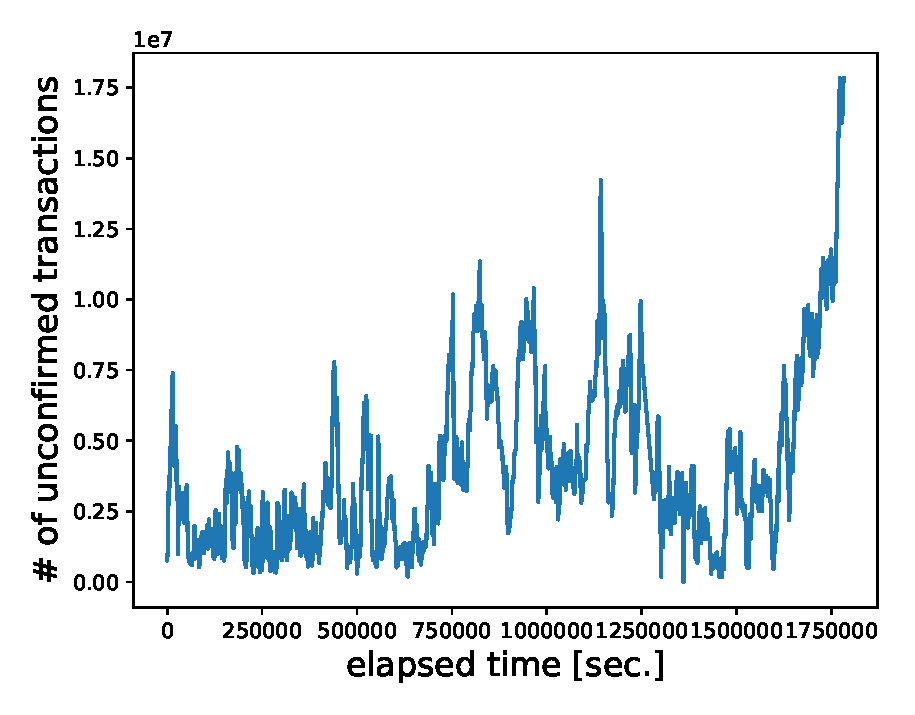
\includegraphics[width=70mm]{time_vs_tx-plot.eps}
  \end{center}
  \vspace{35mm}
  %\caption{STNの未確認取引件数の時間変化}
  \caption{Trend of Unconfirmed Transactions in STN.}
  \label{fig:unconfirmed_tx}
  %  \ecaption{english caption is here}
\end{figure}
%


%この図を作成する元となったデータはwhatsonchain\cite{woc}で報告されているものを収集して利用している.
The data from which this figure is derived are collected and used from whatsonchain\cite{woc}.
%図\ref{fig:unconfirmed_tx}より,定常的に1,000,000以上の取引がTransaction poolに存在していることが分かる.
Figure \ref{fig:unconfirmed_tx} shows that there are regularly more than 1 million transactions in the Transaction pool. 
%また時々,取引数が10,000,000以上に達することも分かる.
It is also found that the number of transactions sometimes reaches more than 10 million.
%BSVではOP\_RETURNスクリプトの利用をサポートしているが,取引内容の大半は単純にアドレス間の送金になっている.
BSV supports the use of OP\_RETURN scripts, but most transactions are simply transfers between addresses.


%STNのネットワークは一般に公開されており,誰でもノードを構築してP2Pネットワークに参加することができる.
The network of STN is open to the public, and anyone can construct a node and participate in P2P network.
%ただしノード構築の為のシステム要求として,CPUは8〜16コア,メモリは64GB(+64GB Swap),ハードディスクは3TB以上,インターネット接続は上り下りとも1Gbit以上の性能が要求されている.
However, as system requirements for node construction, performance of 8--16 cores for CPU, 64 GB (+64 GB Swap) for memory, over 3 TB for hard disk, and over 1 Gbit for both up and down Internet connection are required.
%BCの総容量は2021年2月9日時点で2.4TBとなっている.
The total size of BC was 2.4 TB at that time in February 9, 2021.
%BSVのTestnetでは22GB,Mainnetでも284GB程度である為,比較するとBCの容量が非常に大きいことが分かる.
Since it is about 22 GB in Testnet of BSV and 284 GB in Mainnet, it is proven that the capacity of BC is very large in comparison.
%またSTNのBCのブロック高は2021年2月9日時点で15,216となっており,小さい.これは過去にBCの再編成(=ブロック高を下げて再開)を何度か実施している為である.
And, the block height of BC of STN became 15,216 as of February 9, 2021, and it is small, which is because BC has been reorganized several times in the past.
%BSVのgithubの情報では2020年4月と11月にBCの再編成が行われたことが記録されている.
Information on the github of the BSV records that BC was reorganized in April and November 2020. 



%またシステム要求からも分かるが,STNはCPUによるブロック採掘が可能になっている.
%ブロック採掘の難易度の時間変化を図\ref{fig:difficulty}に示す.
And, block mining by CPU becomes possible in STN, as it is proven from the system requirement.
The time course of block mining difficulty is shown in Fig.~\ref{fig:difficulty}.
%
\begin{figure}[t]
  \vspace{-35mm}
  \begin{center}
    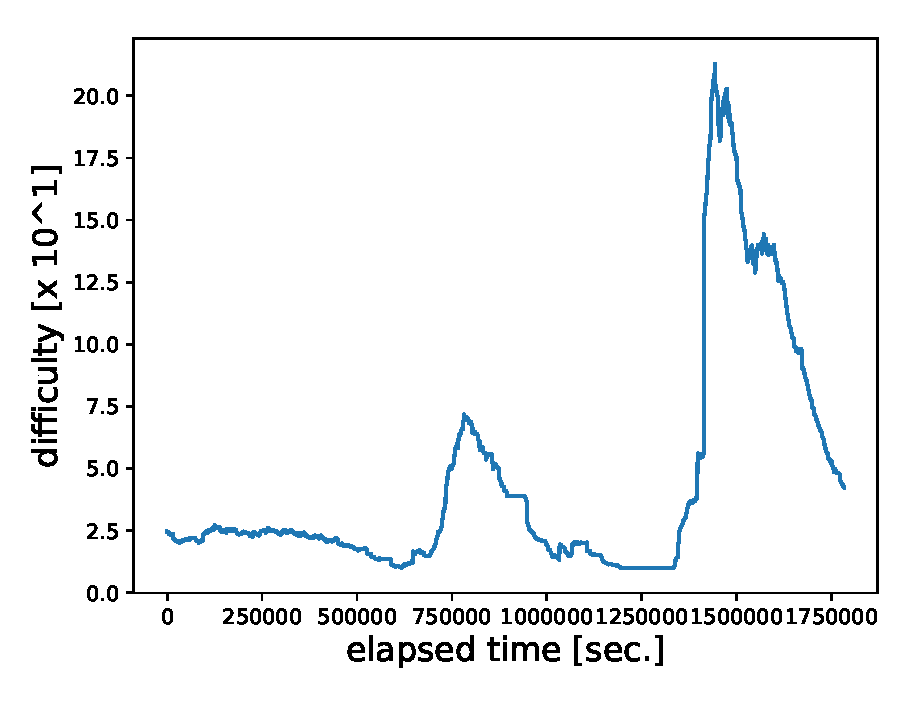
\includegraphics[width=70mm]{time_vs_difficulty-plot.eps}
  \end{center}
  \vspace{35mm}
  %\caption{ブロック採掘の難易度の時間変化}
  \caption{Block mining difficulty over time.}
  \label{fig:difficulty}
  %  \ecaption{english caption is here}
\end{figure}
%
%難易度は1〜数十の範囲で変化しており,容易に採掘が可能となっている.
The degree of difficulty varies from one to several tens, making mining easy.



%STNでは最大ブロックサイズが10GBになるように設定することが推奨されている.
It is recommended that STNs be configured with a maximum block size of 10 GB.
%またBitcoin scriptが使用可能なメモリの上限も2GBに設定することが推奨されている.
It is also recommended that Bitcoin scripts be limited to 2GB of memory.
%これまでに採掘されたブロックのサイズ分布を調べた結果を図\ref{fig:block_size}に示す.
Figures \ref{fig:block_size} show the results of examining the size distribution of blocks mined so far.
%
\begin{figure}[t]
  \vspace{-35mm}
  \begin{center}
    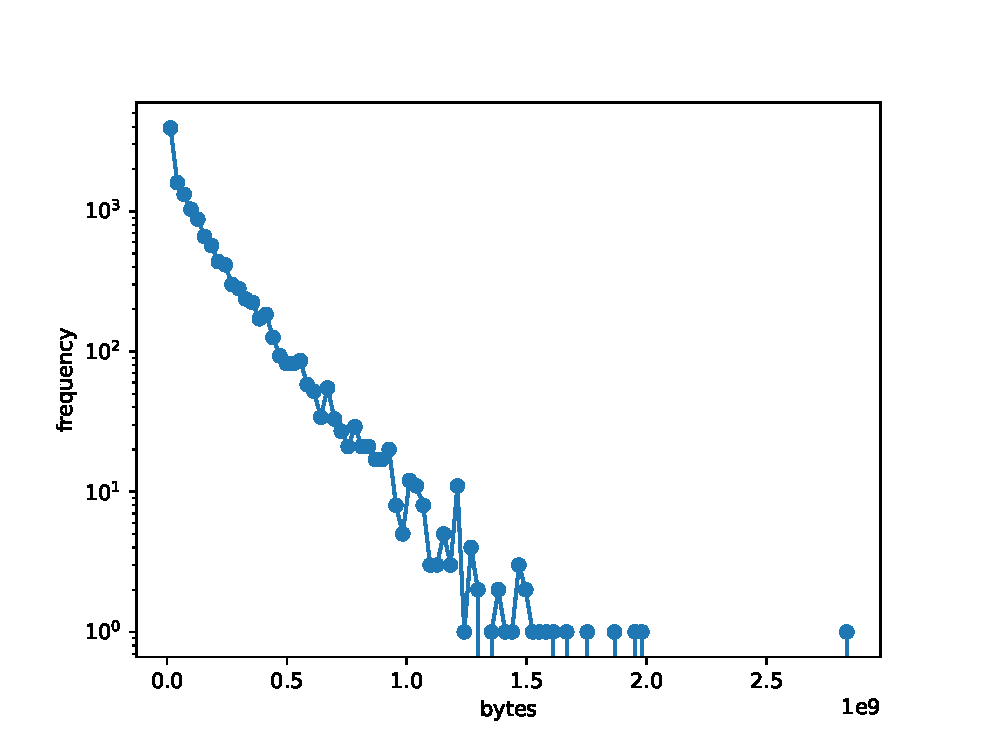
\includegraphics[width=70mm]{bsv_stn-block_bytes-semilogy2.eps}
    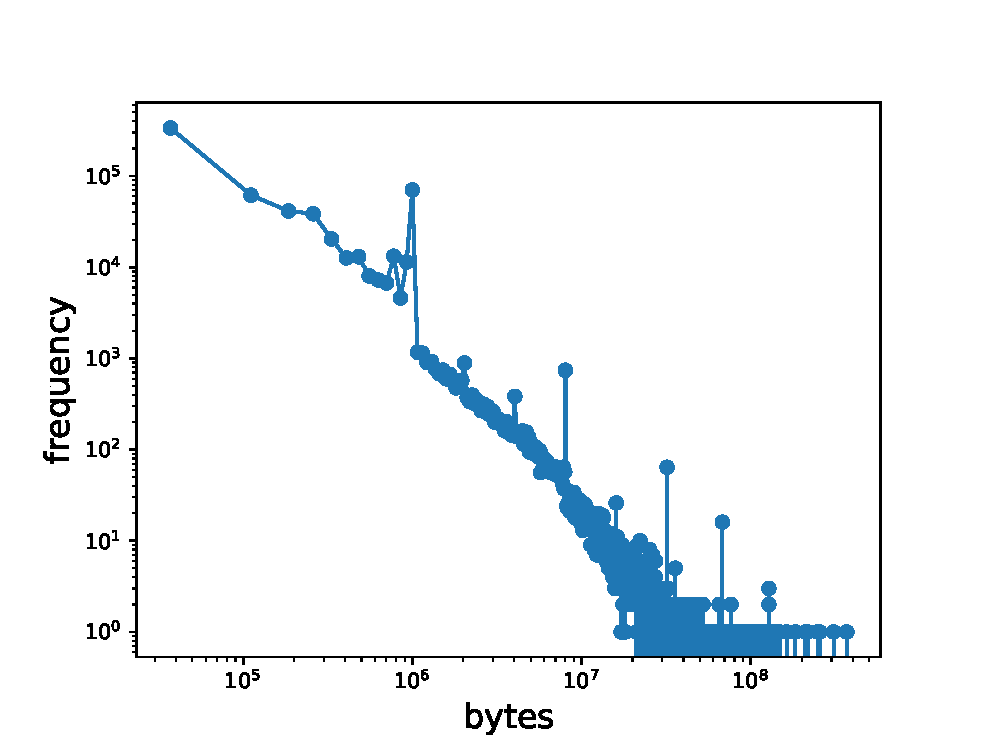
\includegraphics[width=70mm]{bsv_mainnet-block_bytes-loglog.eps}
  \end{center}
  \vspace{35mm}
  %\caption{Bitcoin SVにおけるブロックサイズ分布(上図はSTN,下図はMainnet)}
  \caption{Block Size Distribution in Bitcoin SV (Above is STN, below is Mainnet).}
  \label{fig:block_size}
  %  \ecaption{english caption is here}
\end{figure}
%
%STNのブロックサイズ分布は指数分布に従っているように見える.
The block size distribution of STN seems to follow an exponential distribution.
%またこれまでに採掘された最大ブロックサイズは2.9GBになっている.
The largest block size ever mined was 2.9 GB.
%一方,図\ref{fig:block_size}の下図はMainnetでのブロックサイズ分布になるが,興味深いことに指数分布よりも冪分布に従っているように見える.
On the other hand, the figure below in Figs.~\ref{fig:block_size} shows the block size distribution in Mainnet, which interestingly seems to follow a power distribution rather than an exponential distribution.
%また冪指数の傾向からPareto-Zipf則(=冪指数2の冪分布)に従っているようにも見える.
It also seems to follow the Pareto-Zipf law (= the power-law distribution of the exponent 2) from the tendency of power exponent. 
%STNのコインには市場価値はないが,Mainnetでは市場価値を持つ.
STN coins have no market value, but Mainnet has a market value.
%分布にこのような差が生まれる理由については,よく分かっていないが,市場価値を持つコインが入手できる場合,何らかの経済原理が働くことが影響していると考えられる.
Though the reason of such difference in the distribution is not well understood, it seems to be influenced by some economic principle when coins with market value are available.


%BSVは採掘者の評判を評価する観点から採掘したブロックに採掘者IDを記録することを推奨している.
The BSV recommends recording the miner ID on the blocks mined to assess the reputation of the miner.
%この採掘者IDを参考にしてブロック採掘頻度のランキングを計算した結果を図\ref{fig:minerrank}に示す.
Figures \ref{fig:minerrank_stn} and \ref{fig:minerrank_mainnet} show the results of calculating the ranking of block mining frequency with reference to this miner ID.
%
\begin{figure}[t]
  \vspace{-35mm}
  \begin{center}
    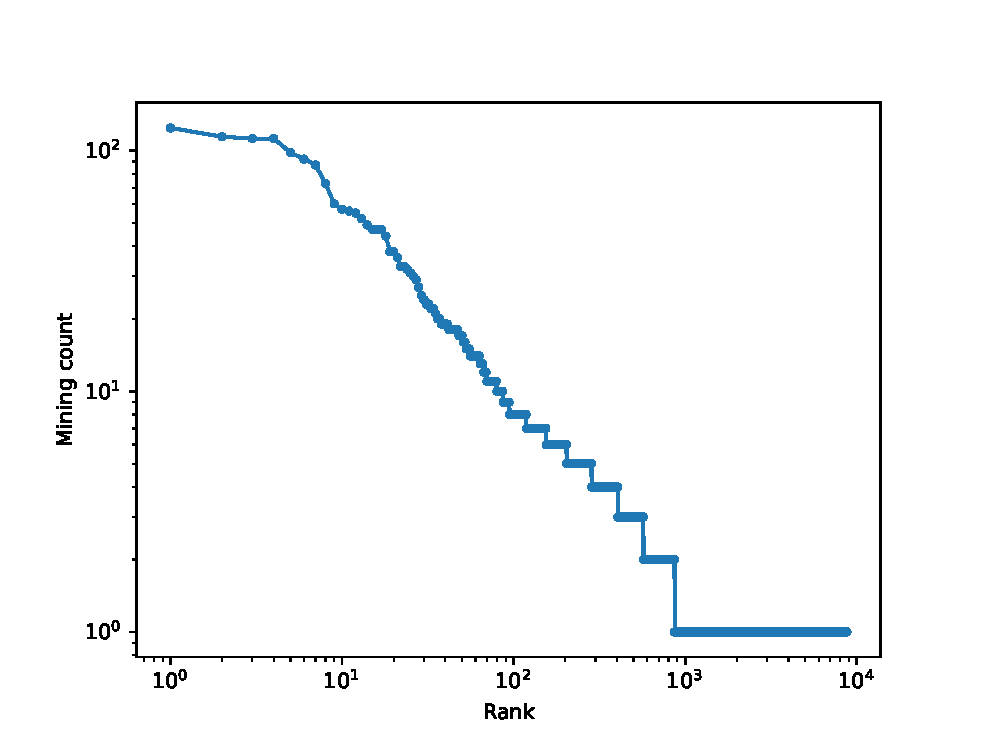
\includegraphics[width=70mm]{bsv_stn-block_miners-ranking-loglog.eps}
  \end{center}
  \vspace{35mm}
  %\caption{採掘者IDを参考にして計算したブロック採掘頻度ランキング(STN)}
  \caption{Block mining frequency ranking calculated with reference to miner ID (STN)}
  \label{fig:minerrank_stn}
  %  \ecaption{english caption is here}
\end{figure}
%
%
\begin{figure}[t]
  %\vspace{-35mm}
  \begin{center}
    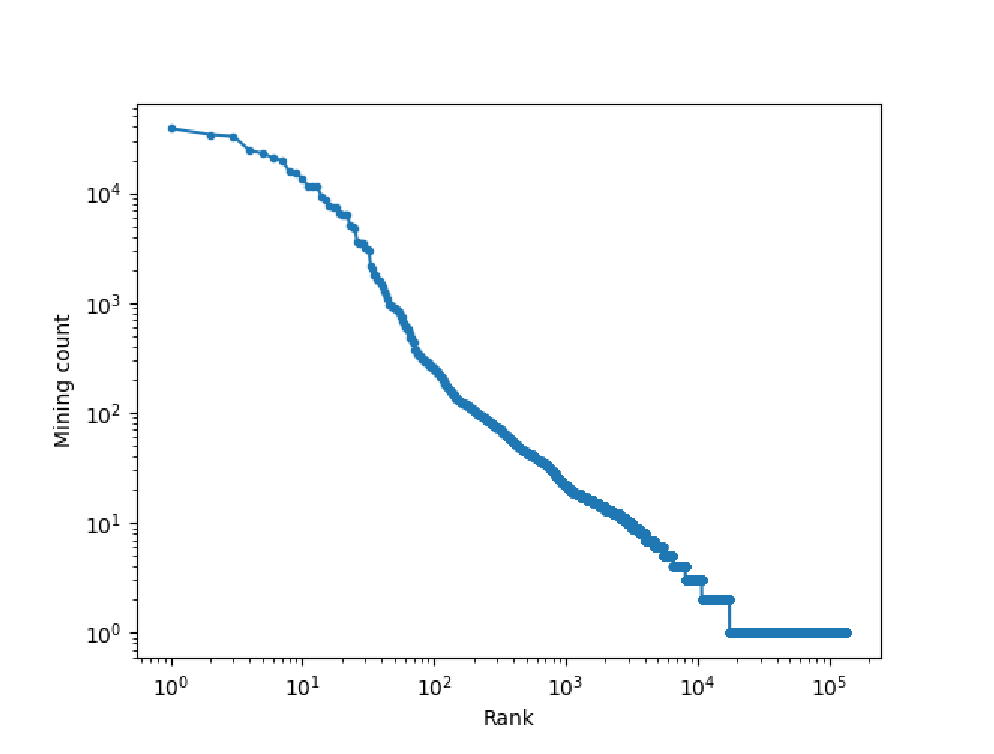
\includegraphics[width=70mm]{bsv_mainnet-block_miners-ranking-loglog.eps}
  \end{center}
  %\vspace{35mm}
  %\caption{採掘者IDを参考にして計算したブロック採掘頻度ランキング(Mainnet)}
  \caption{Block Mining Frequency Ranking Calculated Based on Miner ID (Mainnet)}
  \label{fig:minerrank_mainnet}
  %  \ecaption{english caption is here}
\end{figure}
%
%こちらはSTNとMainnetの両方とも冪分布に従っていることが確認できる.
Both STN and Mainnet seem to follow a power-law distribution.



\section{Performance Evaluation Experiments}
\label{sec:experiments}

\subsection{Experiment 1: Estimating the Occupancy Rate of Approving Transactions in STN}
\label{sec:occupancyrate}

%図\ref{fig:unconfirmed_tx}における未確認取引件数の時間変化から,STNの稼働率を推定した.
From the time variation of the number of unconfirmed transactions in Fig.~\ref{fig:unconfirmed_tx}, the operating rate of STN was estimated. 
%待ち行列理論に基づいて,STNの推定稼働率$\tilde{\rho}$の時間変化を計算した結果を図\ref{fig:occupancyrate}に示す.
Figure~\ref{fig:occupancyrate} shows the results of calculating the time variation of the estimated STN utilization rate $\tilde{\rho}$ based on queuing theory.
%
\begin{figure}[tb]
  \vspace{-35mm}
  \begin{center}
    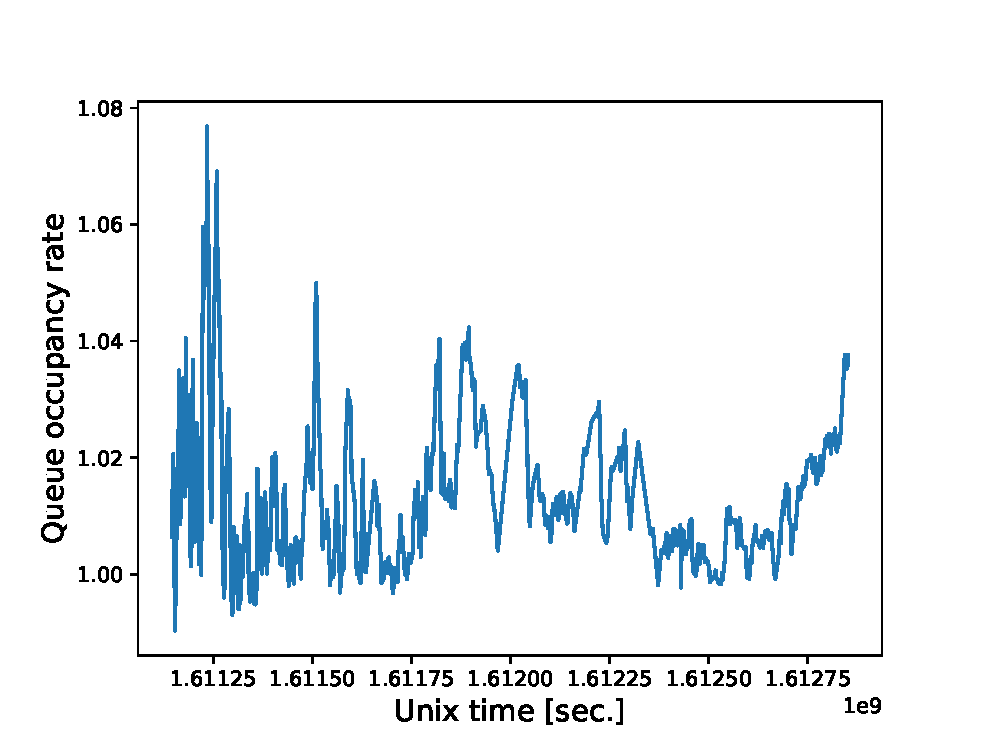
\includegraphics[width=70mm]{bsv_stn-rho-queue_occupancy_rate.eps}
  \end{center}
  \vspace{35mm}
  %\caption{STNの推定稼働率$\tilde{\rho}$の時間変化}
  \caption{Time variation of the estimated occupancy rate in STN $\tilde{\rho}$.}
  \label{fig:occupancyrate}
  %  \ecaption{english caption is here}
\end{figure}
%
%推定稼働率は殆どの時間帯で1を超えていることが分かる.
It can be seen that the estimated occupancy rate exceeds 1 in most time periods. 
%この結果はBCに取り込まれない取引が存在することを示唆している.
This result suggests that there are transactions which are not taken into BC. 
%また2020年11月4日〜2021年2月9日までのデータを用いて推定稼働率の時間平均を取ると$\tilde{\rho} \fallingdotseq 1.04$となった.
Using data from November 4, 2020 to February 9, 2021, the estimated occupancy rate was calculated as $\tilde{\rho} \fallingdotseq 1.04$. 
%この結果より,$1-1/\tilde{\rho} \fallingdotseq 0.0387$の確率でBCに取り込まれない取引が出現していると考えられる.
From these results, it is considered that there is a probability of $1 -1 / \tilde{\rho} \fallingdotseq 0.0387$ that transactions are not included in BC.



\subsection{Experiment 2: Estimating BC Split Probability}
\label{sec:sork}

%STNのノードを構築してP2Pネットワークに接続すると分かるが,大きなブロックが生成されたと思われるタイミングでBCの大きな分岐が起きてSafe modeとなり,bitcoin-cliコマンドを使って送金ができなくなることがある.
If you build an STN node and connect it to a P2P network, you will see that when you think a large block has been created, a large branch of BC will occur and it will go into Safe mode and you will not be able to transfer money using the bitcoin-cli command.
%また一度大きな分岐が起こると解消までに半日近くかかる場合もある.
Once a large bifurcation occurs, it can take nearly half a day to resolve.
%そこでbitcoin-cli getinfoのerrorsの値を取得することで分岐が起きている時間から分岐確率を推定する実験を行った.
We conducted an experiment to estimate the branching probability from the time when the branching occurred by obtaining the errors value of bitcoin-cli getinfo.


%2020年11月4日〜2021年1月13日の期間において,10秒に1回の頻度でerrorsの値を収集した(合計594,880回).
During the period from November 4, 2020 to January 13, 2021, the errors value was collected once every 10 seconds (594,880 times in total).
%またBCが分岐している警告が出た回数を数えた.
We also counted the number of warnings that BC splits.
%その結果,以下の2種類の警告が出た.
As the result, following two kinds of warnings were issued.
%
\begin{itemize}
  \item Warning: The network does not appear to fully agree! We received
        headers of a large fork. Still waiting for block data for more details.
	%(出現頻度は32,724回, 全体に占める割合は約5.5\%)
	(The frequency of occurrence was 32,724 times, accounting for approximately 5.5\% in total.)

  \item Warning: The network does not appear to fully agree! Some miners
        appear to be experiencing issues. A large valid fork has been detected. 
	%(出現頻度は17,782回,全体に占める割合は約3\%)
	(Occurred 17,782 times, accounting for about 3\% in total.)
\end{itemize}
%
%以上の結果より,分岐確率は約$(5.5+3=)8.5$\%と推定することができる.
From these results, we can estimate the bifurcation probability to be about $(5.5 + 3 =) 8.5$\%.
%これはBTCの約2\%の4倍超であることが分かる.
This is about four times larger than the BC-split probability in BTC. 
%ちなみに同じ手法でBSV Mainnetの分岐確率を評価すると0\%となった.
By the way, when the split probability of BSV Mainnet was evaluated by the same method, it became 0\%.
%また,式(\ref{eq:exp})において$F(t)=0.085$と$\lambda=1/600$を代入した時,$t=\tau_{fork} \fallingdotseq 53$秒となることから,STNにおける平均ブロック転送時間は約53秒になっていると推定することができる.
And, when $F(t) = 0.085$ and $\lambda = 1/600$ are substituted in the expression (\ref{eq:exp}), $t = \tau_{fork} \fallingdotseq 53$ seconds, so that the average block transfer time in STN can be estimated to be about 53 seconds.



\subsection{Experiment 3: Testing Transaction Processing Performance}
\label{sec:method}

%常に沢山の取引がTransaction poolにある状況で,取引がBCに取り込まれるまでにどの程度の時間がかかるかを実験により性能評価した.
In this paper, we experimentally evaluate how long it takes for transactions to be incorporated into BC in the situation that there are always many transactions in the transaction pool.a
%実験期間を2021年1月7〜14日の1週間に設定し,期間中に分岐による取引送信ができない場合を除いて常に1分に1回の頻度で,前の1分間にFlightradar24 \cite{flightradar24} のADS-Bデータの収集ノードから千葉工業大学のある津田沼周辺を飛行する民間航空機の位置情報を収集し,OP\_RETURNスクリプトとしてデータを含めた取引の送信を行った.
The experimental period was set for 1 week from January 7 to 14, 2021, and the position information of the civil aircraft which flew around Tsudanuma where Chiba Institute of Technology is located was collected from the collection node of ADS-B data of Flightradar 24 \cite{flightradar24} at the frequency of 1 minute always except for the case in which the transaction transmission by the branch is not possible during the period, and the transaction including the data was transmitted as OP\_RETURN script.
%1取引あたりのサイズは63KB未満になるようにした.
The size per transaction should be less than 63 KB.
%また取引手数料は0.001BSVに固定した.
The transaction fee was fixed at 0.001 BSV.
%ちなみにBSVの取引手数料は1 satoshi/byte以上となっている.
BSV charges more than 1 satoshi/byte.
%昼間は民間航空機が多く飛行する為,取引データのサイズが大きくなるが,夜間は殆ど飛行がない為,書き込むデータが無かった場合は取引の送信は行わなかった.
The size of transaction data is large because many commercial aircrafts fly in the daytime, but transactions are not transmitted when there is no data to write, because there is almost no flight at night.
%実験結果に関するその他の詳細情報はGithub に掲載した
Additional details about the results are available on our Github website 
\footnote{\url{https://github.com/cit-fujihalab/stn_experiments}}.



%実験期間の経過時間と取引が取り込まれたブロック番号の対応関係を図\ref{fig:exp3-1}に示す.
Figure~\ref{fig:exp3-1} shows the correspondence between the elapsed time of the experiment period and the block number in which the transaction was captured. 
%
\begin{figure}[tb]
  %\vspace{-35mm}
  \begin{center}
    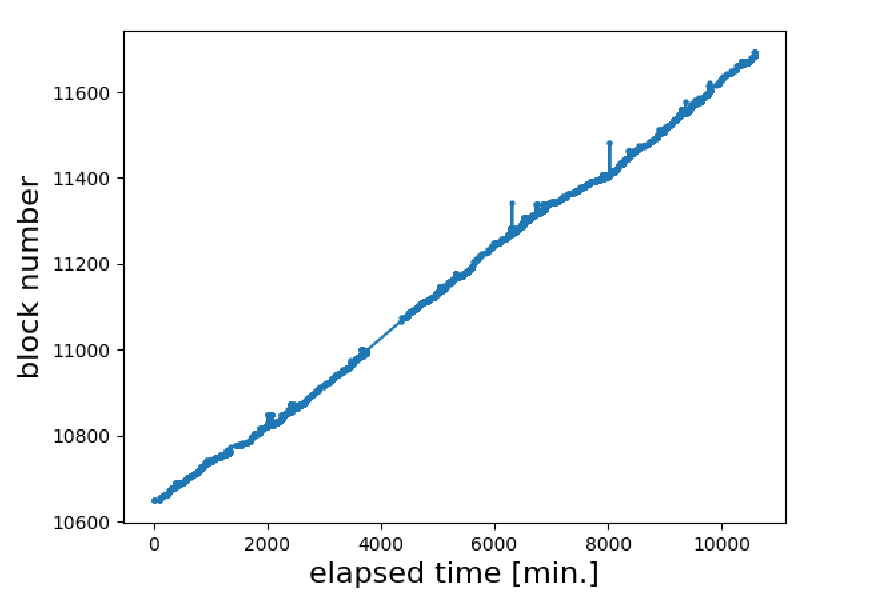
\includegraphics[width=70mm]{exp3-1.eps}
  \end{center}
  %\vspace{35mm}
  %\caption{経過時間と取引が取り込まれたブロック番号の対応関係}
  \caption{Correspondence between the elapsed time and the block number where the transaction was captured.}
  \label{fig:exp3-1}
  %  \ecaption{english caption is here}
\end{figure}
%
%経過時間と共に取引が定期的にブロックに取り込まれていることが確認できる.
You can see that transactions are regularly captured in blocks over time.
%一方,たまになかなかBCに取り込まれない取引があることも確認できる.
On the other hand, it can be confirmed that there are some transactions which are seldom taken into BC.


%実験期間中に合計6,828取引を送信したが,そのうち104取引はBCに取り込まれなかった.
A total of 6,828 transactions were sent during the experimental period, 104 of which were not incorporated into BC.
%このことより,取引がBCに取り込まれない確率が$(104/6828 \fallingdotseq) 0.02$と計算できる.
From this, the probability that the transaction does not get into BC can be calculated as $(104/6828 fallingdotseq) 0.02$.
%この結果は\ref{sec:occupancyrate}節で計算した$1-1/\tilde{\rho} \fallingdotseq 0.0387$の確率でBCに取り込まれない取引が出現していると推定した結果とほぼ同じ値になっていることが確認できる.
This result is almost the same as the result calculated in Fig.~\ref{sec:occupancyrate} clause, which estimates that there is a probability of $1 -1 / \tilde{\rho} \fallingdotseq 0.0387$ that transactions are not approved. 


%次に取引送信からBCに取り込まれるまでにかかる時間のヒストグラムを図\ref{fig:exp3-2}に示す.
A histogram of the time taken from transaction transmission to incorporation into BC is shown in Fig.~\ref{fig:exp3-2}.
%
\begin{figure}[t]
  %\vspace{-35mm}
  \begin{center}
    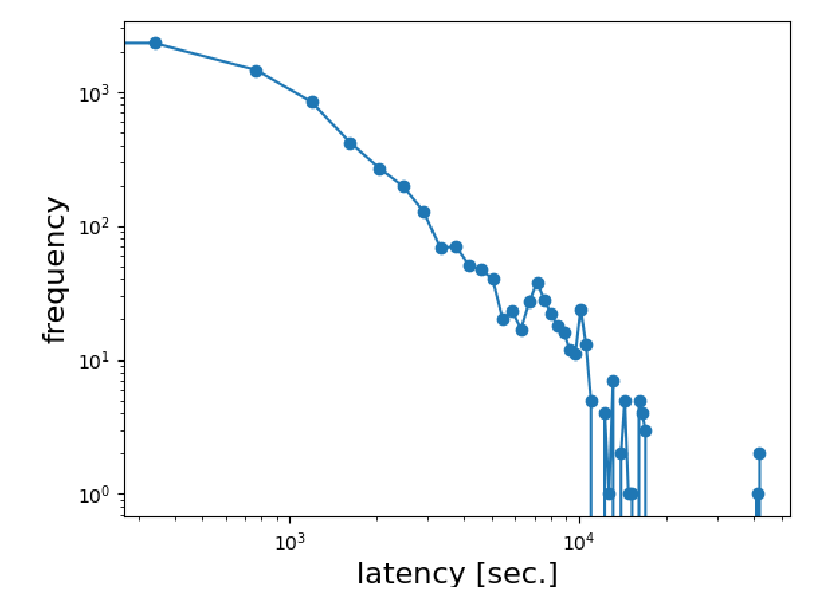
\includegraphics[width=70mm]{exp3-2.eps}
  \end{center}
  %\vspace{35mm}
  %\caption{取引送信からBCに取り込まれるまでにかかる時間のヒストグラム}
  \caption{Histogram of latency time of transaction to be taken into BC.}
  \label{fig:exp3-2}
  %  \ecaption{english caption is here}
\end{figure}
%
%ブロック生成時間分布が指数分布に従うことから,半日程度の短期間ではBCに取り込まれる時間は指数分布に従うが,1週間程度の長期間になると指数分布から外れてくる.
Since the block generation time distribution follows the exponential distribution, the time taken into BC follows the exponential distribution in the short term of about half a day, but it deviates from the exponential distribution in the long term of about one week.
%実際に図\ref{fig:exp3-2}のとおり両対数プロットで直線的な傾向が現れる為,冪分布に従う傾向が現れていることが確認できる.
In fact, as shown in Fig.~\ref{fig:exp3-2}, a linear trend appears in the double-logarithmic plot, which confirms that the trend follows the power distribution.
%また冪指数を両対数プロットの傾きから見積もると3/2に近いことが分かる.
The power index is estimated from the slope of the double-logarithm plot and is close to 3/2.
%これらの結果は優先権付き待ち行列の理論解析結果と矛盾しない.
These results are consistent with the theoretical analysis of priority queueing.
%このことから手数料の低い取引が優先度が低くなり,BCに取り込まれるまでに時間がかかっていることが予想される.
From this fact, it is anticipated that the transaction with low commission becomes low priority, and that it takes time to be taken into BC.



%取引サイズに対する取引手数料の割合と取引がBCに取り込まれるまでにかかった時間の関係を図\ref{fig:exp3-3}に示す.
Figure \ref{fig:exp3-3} shows the relationship between the ratio of transaction fees to transaction size and the latency time until a transaction is approved. 
%
\begin{figure}[t]
  %\vspace{-35mm}
  \begin{center}
    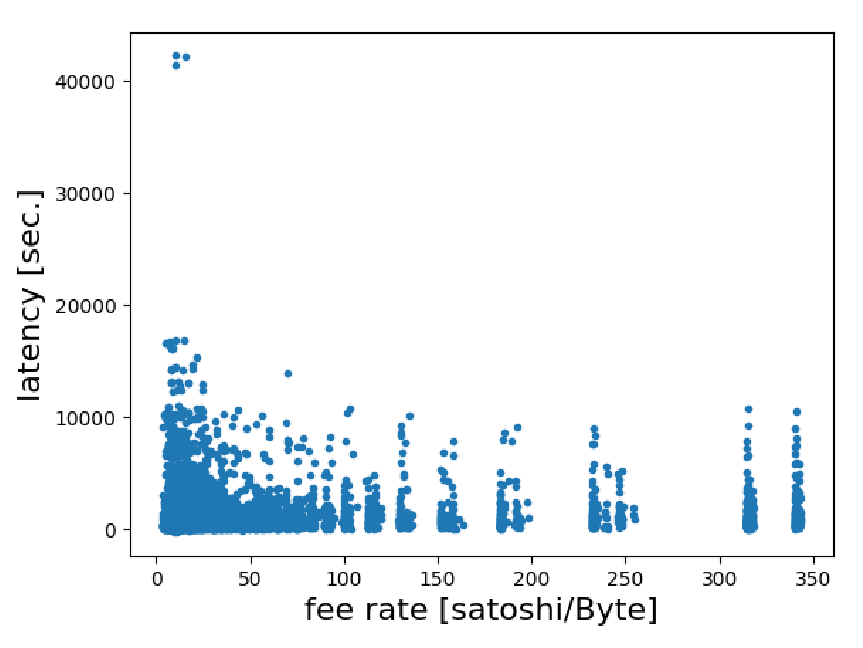
\includegraphics[width=70mm]{exp3-3.eps}
  \end{center}
  %\vspace{35mm}
  %\caption{取引サイズに対する取引手数料の割合と取引がBCに取り込まれるまでにかかった時間の関係}
  \caption{Relationship between the transaction fee as a percentage of transaction size and the time it takes for the transaction to arrive in BC.}
  \label{fig:exp3-3}
  %  \ecaption{english caption is here}
\end{figure}
%
%割合(fee rate)が低いとBCに取引が取り込まれるまでに時間がかかっていることが分かる.
A low fee rate indicates that it is taking a long time for transactions to be incorporated into BC.
%このことからSTNにおいても優先権付き待ち行列理論による考察は有効であると考えられる.
Therefore, it is considered that the consideration by the queueing theory with priority is effective even in STN.



\section{Conclusion}
\label{sec:conclusion}

%本研究ではBitcoin STNのノードを構築し,ブロックサイズの上限を撤廃した環境における取引処理に関するデータ分析や性能評価実験を行った.
In this study, a Bitcoin STN node was constructed, and data analysis and performance evaluation experiment on transaction processing in the environment in which the block size upper limit was removed were carried out.
%取引処理の稼働率の時間変化を調べた結果,推定稼働率は殆どの時間帯において1を超えていることが分かった.
As a result of examining the time variation of the working rate of transaction processing, it was proven that the estimated working rate exceeded 1 in most time zones.
%bitcoin-cliの機能を用いてBCの分岐確率の推定も行った結果,STNでは約8.5\%となり,BTCの4倍超の確率となっていることが分かった.
Using bitcoin-cli, we also estimated the branching probability of BC, and found that it is about 8.5\% for STN, which is more than 4 times the probability of BTC.
%またP2Pネットワークの平均ブロック転送時間も約53秒と推定できた.
The average block transfer time of the P2P network was also estimated to be about 53 seconds.
%OP\_RETURNスクリプトを含む取引を1分に1回の高頻度で1週間の期間,転送することで取引処理性能を実験的に評価した.
The transaction processing performance was experimentally evaluated by transferring transactions containing OP\_RETURN scripts at a high frequency of once a minute for a period of one week.
%その結果,取引がBCに取り込まれる確率は98\%であり,その時間分布は長期的には冪分布に従うような傾向が確認できた.
As a result, it was found that the probability of transactions being incorporated into BC was 98\%, and its time distribution tended to follow the power distribution in the long term.
%また優先権付き待ち行列の理論と矛盾しない3/2の冪指数に従う傾向も確認できた.
We also confirmed the tendency to follow a power exponent of 3/2, which is consistent with the theory of priority queueing.
%このことからSTNにおいても優先権付き待ち行列理論による考察は有効であると言える.
From this fact, it can be said that the consideration by the queueing theory with priority is effective even in STN.


%今後の課題としては,より大量な数の取引を長期間に渡って送信し続けた時の処理性能について確認することが挙げられる.
For future work, it is necessary to confirm the processing performance when a larger number of transactions are continuously transmitted over a long period of time.




\begin{acknowledgement}
 This work was partially supported by the Japan Society for the Promotion of 
Science (JSPS) through KAKENHI (Grants-in-Aid for Scientific Research) Grant 
Number 20K11797. 
\end{acknowledgement}



%%
%\section*{Appendix}
%\addcontentsline{toc}{section}{Appendix}
%%
%%




\begin{thebibliography}{99}

% Blockchain
\bibitem{HS1991}
  S. Haber and W. S. Stornetta, 
  ``How To Time-Stamp a Digital Document,''
  J. Cryptology, 3, 99-111 (1991)
  %\url{https://link.springer.com/content/pdf/10.1007\%2FBF00196791.pdf}

\bibitem{BHS1993}
  D. Bayer, S. Haber, and W. S. Stornetta,
  ``Improving the Efficiency and Reliability of Digital Time-Stamping,''
  Sequences II: Methods in Communication, Security, and Computer Sicence, 
  pp. 329-334 (1993).

\bibitem{HS1997}
  S. Haber and W. S. Stornetta, 
  ``Secure Names for Bit-Strings,''
  CCS'97: Proceedings of the 4th ACM conference on Computer and 
  communications security, pp. 28-35 (1997).
  %\url{https://nakamotoinstitute.org/static/docs/secure-names-bit-strings.pdf}


% Bitcoin
\bibitem{nakamoto}
  S. Nakamoto, 
  ``Bitcoin: A Peer-to-Peer Electronic Cash System''
  (White paper), 2008 
  \url{https://bitcoin.org/bitcoin.pdf}
  \url{https://www.bitcoinsv.io/bitcoin.pdf}


% Proof of Work
\bibitem{DN1993}
  C. Dwork and M. Naor, 
  ``Pricing via Processing or Combatting Junk Mail,''
  Advances in Cryptology (CRYPTO'92), 
  Lecture Notes in Computer Science, vol. 740, Springer (1993). 
  %\url{https://web.cs.dal.ca/~abrodsky/7301/readings/DwNa93.pdf}


\bibitem{JJ1999}
  M. Jakobsson and A. Juels, 
  ``Proofs of Work and Bread Pudding Protocols (Extended Abstract),''
  In: Preneel B. (eds) Secure Information Networks, 
  The International Federation for Information Processing, 
  vol 23, Springer (1999).
  %\url{https://www.arijuels.com/wp-content/uploads/2013/09/PoW.pdf}


\bibitem{btc}
  Bitcoin Core 
  \url{https://github.com/bitcoin/bitcoin}


% scalability problem
\bibitem{ZHZB2020}
  Q. Zhou, \textit{et al.}, 
  ``Solutions to Scalability of Blockchain: A Survey''
  IEEE Access, Vol. 8, pp.16440-16455, IEEE, 2020. 


\bibitem{Fujihara2018}
  A. Fujihara,
  ``Proposing a System for Collaborative Traffic Information Gathering and 
  Sharing Incentivized by Blockchain Technology,''
  The 10th International Conference on Intelligent Networking and 
  Collaborative Systems (INCoS-2018), pp.170-182 (2018)
  \url{https://link.springer.com/chapter/10.1007/978-3-319-98557-2_16}

\bibitem{Fujihara2019}
  A. Fujihara,
  ``PoWaP: Proof of Work at Proximity for a crowdsensing system for 
  collaborative traffic information gathering,'' 
  Internet of Things, 100046, Elsevier (2019).
  \url{https://www.sciencedirect.com/science/article/pii/S254266051830177X}

\bibitem{Fujihara2020}
  A. Fujihara, 
  ``Proposing a Blockchain-Based Open Data Platform and Its Decentralized Oracle,''
  Advances in Intelligent Networking and Collaborative Systems (INCoS2019), 
  Advances in Intelligent Systems and Computing, 
  Vol. 1035, pp. 190--201, Springer (2020).
  \url{https://link.springer.com/chapter/10.1007/978-3-030-29035-1_19}

\bibitem{YF2021a}
  T. Yanagihara and A. Fujihara, 
  ``Considering Cross-Referencing Method for Scalable Public Blockchain,''
  Advances in Internet, Data and Web Technologies, 
  Lecture Notes on Data Engineering and Communications Technologies, 
  Vol. 65, pp. 220-231, Springer (2021). 
  \url{https://link.springer.com/chapter/10.1007/978-3-030-70639-5_21}

\bibitem{YF2021b}
  T. Yanagihara and A. Fujihara,
  ``Cross-Referencing Method for Scalable Public Blockchain,''
  Internet of Things, Vol. 15, 100419 (2021). 
  \url{https://www.sciencedirect.com/science/article/pii/S2542660521000639}


\bibitem{PD2016}
  J. Poon and T. Dryja, 
  ``The Bitcoin Lightning Network: Scalable Off-Chain Instant Payments,'' 
  (2016) \url{https://lightning.network/lightning-network-paper.pdf}


\bibitem{silkroad}
  FBI, 
  ``Manhattan U.S. Attorney Announces Seizure of Additional \$28 Million 
    Worth of Bitcoins Belonging to Ross William Ulbricht, Alleged Owner 
    and Operator of ``Silk Road'' Website, '' 2013.
  \url{https://archives.fbi.gov/archives/newyork/press-releases/2013/manhattan-u.s.-attorney-announces-seizure-of-additional-28-million-worth-of}\\
  \url{-bitcoins-belonging-to-ross-william-ulbricht-alleged-owner-and}\\
  \url{-operator-of-silk-road-website}

\bibitem{alphabay}
  The US Department of Justice,
  ``AlphaBay, the Largest Online 'Dark Market,' Shut Down,'' 2017.
  \url{https://www.justice.gov/opa/pr/alphabay-largest-online-dark-market-shut-down}

\bibitem{welcome2video}
  The US Department of Justice,
  ``South Korean National and Hundreds of Others Charged Worldwide in the Takedown 
    of the Largest Darknet Child Pornography Website, Which was Funded by Bitcoin,'' 
  2019.
  \url{https://www.justice.gov/opa/pr/south-korean-national-and-hundreds-others-charged-worldwide}\\
  \url{-takedown-largest-darknet-child}



\bibitem{bloX}
  U. Klarman, \textit{et al.},
  ``bloXroute: A Scalable Trustless Blockchain Distribution Network''
  (White paper), 2018.
  \url{https://bloxroute.com/wp-content/uploads/2018/03/bloXroute-whitepaper.pdf}


\bibitem{bsv}
  Bitcoin SV (Satoshi Vision) 
  \url{https://github.com/bitcoin-sv/bitcoin-sv}

\bibitem{bitcoinscaling}
  Bitcoin Scaling Test Network
  \url{https://bitcoinscaling.io/}




\bibitem{OB2005}
  J. G. Oliveira and A.-L. Barab\'asi,
  ``Darwin and Einstein correspondence patterns,'' 
  Nature 437, 1251, 2005.


\bibitem{KK2019}
  S. Kasahara and J. Kawahara,
  ``Effect of Bitcoin fee on transaction-confirmation process,''
  Journal of Industrial and Management Optimization, 15 (1): 365-386, 2019.


\bibitem{woc}
  WhatsOnChain.com, BSV Explorer - STN,
  \url{https://stn.whatsonchain.com/}



% Flightradar24
\bibitem{flightradar24}
  Flight Tracker | Flightradar24 | Track Planes in Real-time,
  \url{https://www.flightradar24.com/}



\end{thebibliography}

\end{document}
